\section{Performance Analysis}
In this first version of the report we focus on studying the completion time as function of the parallelism degree. For each algorithm, we run single-shot computations (that is, the ones that do not work on streams of data sets to sort), each of them varies from the others for the parallelism degree (it doubles at each execution). Another degree of freedom is represented by the size of the data set: we refer to ''small'', ''large'' or ''huge'' data sets for sizes that are respectively of the order of KBs, MBs and (at least) GBs. At the present moment, in order to keep limited the complexity of this first performance study, we decide to fix the seed needed to generate the data set.

\subsection{Pianosa}
Pianosa is not obviously the ideal platform to run our tests: for instance, it suffers the lack of both shared memory machines and a powerful interconnection networks (MPI relies on top of TCP/IP over Ethernet). It could be anyway a good starting point for the performance analysis if we take care of the fact that the architecture has a lot of native limitations that may \textit{significantly} affect the performance. We analyze the behavior of our algorithms for large data sets, while the case of small data sets will be treated in the following section; huge data sets will be analyzed in the final version of the report (at the present moment the framework still needs some features to be implemented in order to manage huge data sets).

\subsubsection*{Large data sets}
In our test we run a lot of computations that differ each other for the following parameters:
\begin{itemize}
\item algorithm $\in \lbrace ANSI\ qsort$, $Bitonicsort$, $Samplesort$, $Bucketsort$, $Mergesort$, $K$-$Way$ $Mergesort$, $Load$-$Balanced$ $Mergesort$, $Load$-$Balanced$ $Multi$-$Way$ $Mergesort$ $\rbrace$;
\item parallelism degree $\in \lbrace 2,\ 4,\ 8,\ 16 \rbrace$;
\item size of the data set $\in \lbrace 10,\ 50,\ 100,\ 200,\ 400 \rbrace \ MBs$.
\end{itemize} 
Figure~\ref{large-tc} shows the completion time for sorting large data sets. One thing is clearly visible: for parallelism degrees up to 8, sequential $qsort$ even outperforms almost all the algorithms; for parallelism degree 16 some algorithms improve a little the completion time ($Samplesort$, $Bucketsort$, $Mergesort$, $Load$-$Balanced$ $Multi$-$Way$ $Mergesort$), but anyway it keeps to be very close (same order magnitude) to the one of $qsort$. However, this result is not really surprising. Indeed, as we told in advance, we must take care of the following features:
\begin{itemize}
\item the computation performed on each element of the data set has fine grain;
\item the whole data set is of the order of MBs. In the best case, changing the parallelism degree from $2$ to $4$ (or at most from $4$ to $8$) and assuming a data set size of $400$ MB, we notice that almost all parallel algorithms significatively (but not ideally) improve the completion time. This is because each process can work on a portion of data that is still roughly a hundred of MBs. In all other cases, each process works on very smaller portion of data, so the parallelization, given that the computation on each element has fine grain, is not so useful. 
\item the cost and the number of communications that, as we saw in~\ref{test-env-pianosa}, may impact the completion time. We will further investigate and detail the impact of communications in the final version of the report.
\end{itemize}
These consideration aims at justifying the non-ideal scalability of the algorithms. We hope that for huge data sets we will be able to improve these results by increasing the time spent by each process on the sequential computation, hoping that it will be relatively larger than the one spent in communications. Surely, at least the difference between the time completion of parallel algorithms and the one of sequential qsort will become significant.
\begin{figure}[p]
	\centering
	\subfloat[Cost of sequential qsort.]{\label{large-sequential}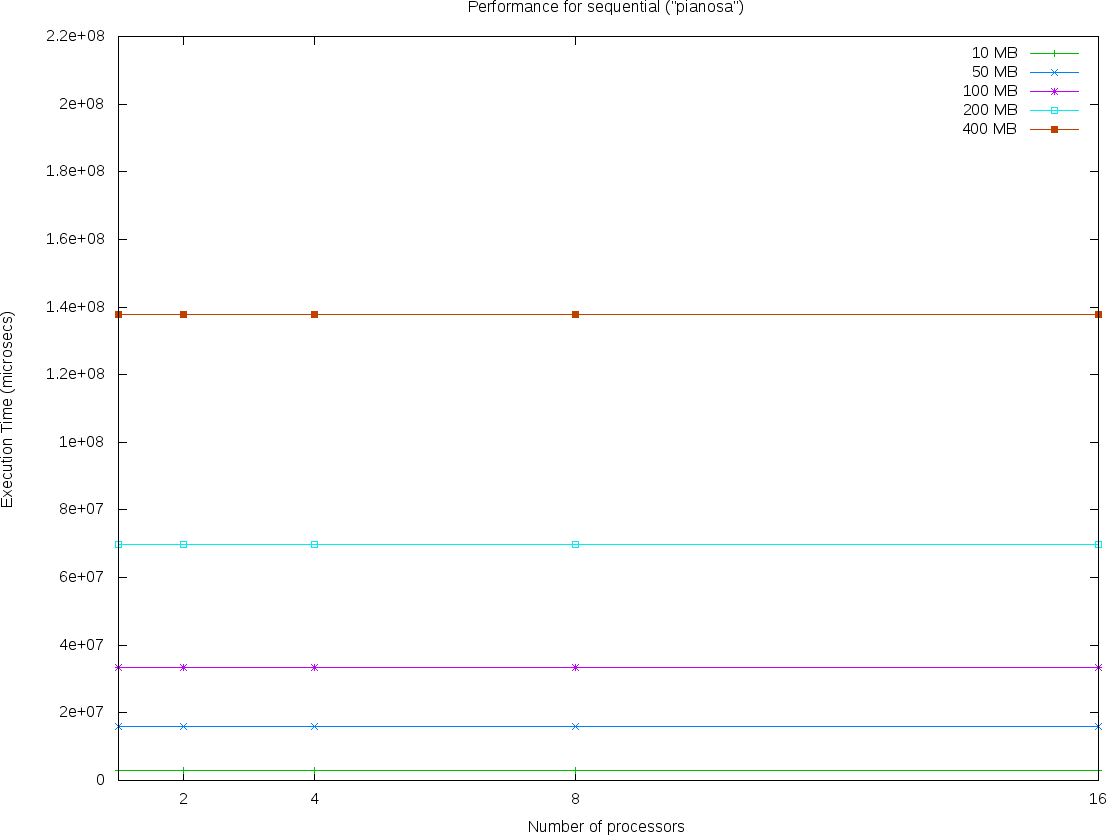
\includegraphics[width=0.4\textwidth]{results/large_sequential_pianosa}} 
	\hspace*{20pt}	
  	\subfloat[Bitonicsort.]{\label{large-bitonicsort}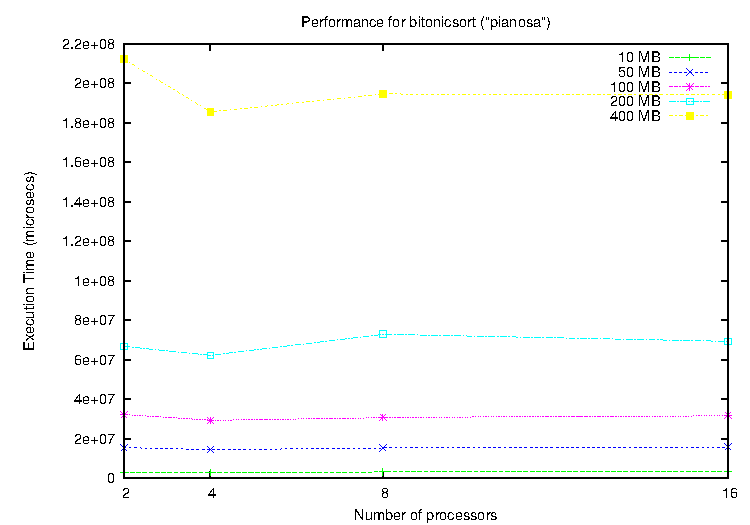
\includegraphics[width=0.4\textwidth]{results/large_bitonicsort_pianosa}}
  		
	\centering
	\subfloat[Bucketsort.]{\label{large-bucketsort}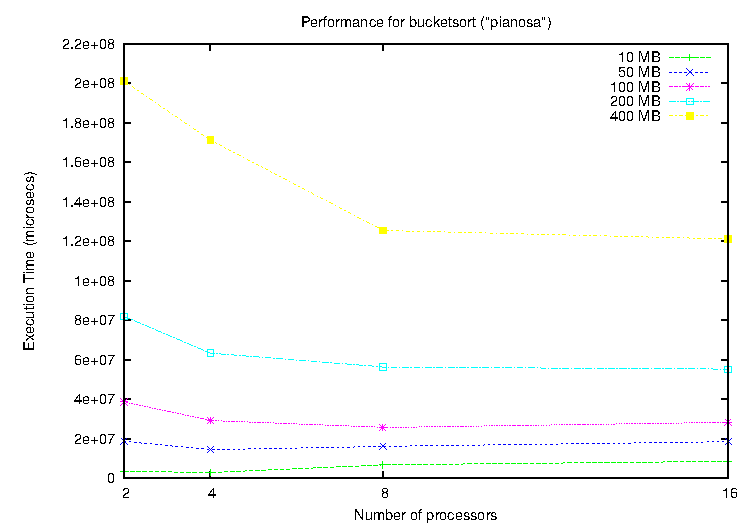
\includegraphics[width=0.4\textwidth]{results/large_bucketsort_pianosa}}  
  	\hspace*{20pt}
  	\subfloat[Samplesort.]{\label{large-samplesort}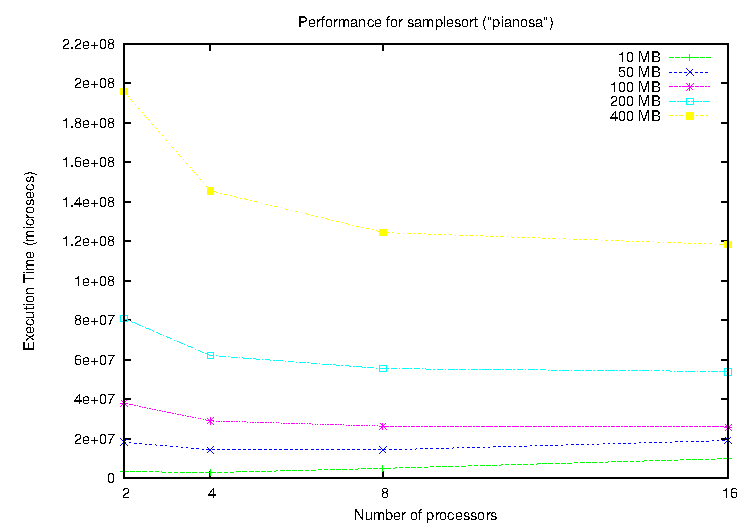
\includegraphics[width=0.4\textwidth]{results/large_samplesort_pianosa}}  
	
	\centering
  	\subfloat[Mergesort.]{\label{large-mergesort}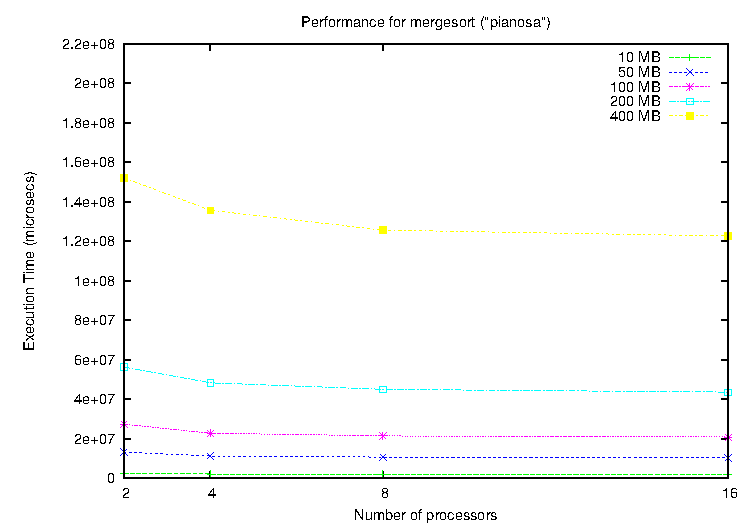
\includegraphics[width=0.4\textwidth]{results/large_mergesort_pianosa}}  
  	\hspace*{20pt}  
  	\subfloat[K-Way Mergesort.]{\label{large-kmerge}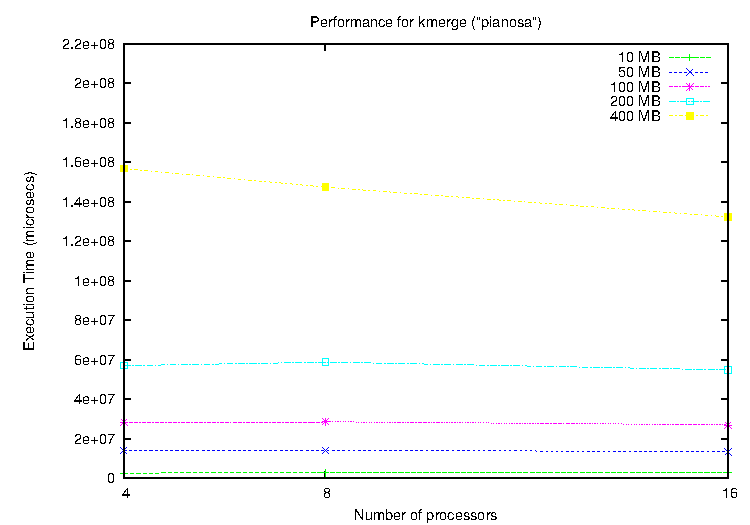
\includegraphics[width=0.4\textwidth]{results/large_kmerge_pianosa}} 
	
	\centering
  	\subfloat[Load-Balanced Mergesort.]{\label{large-lbmergesort}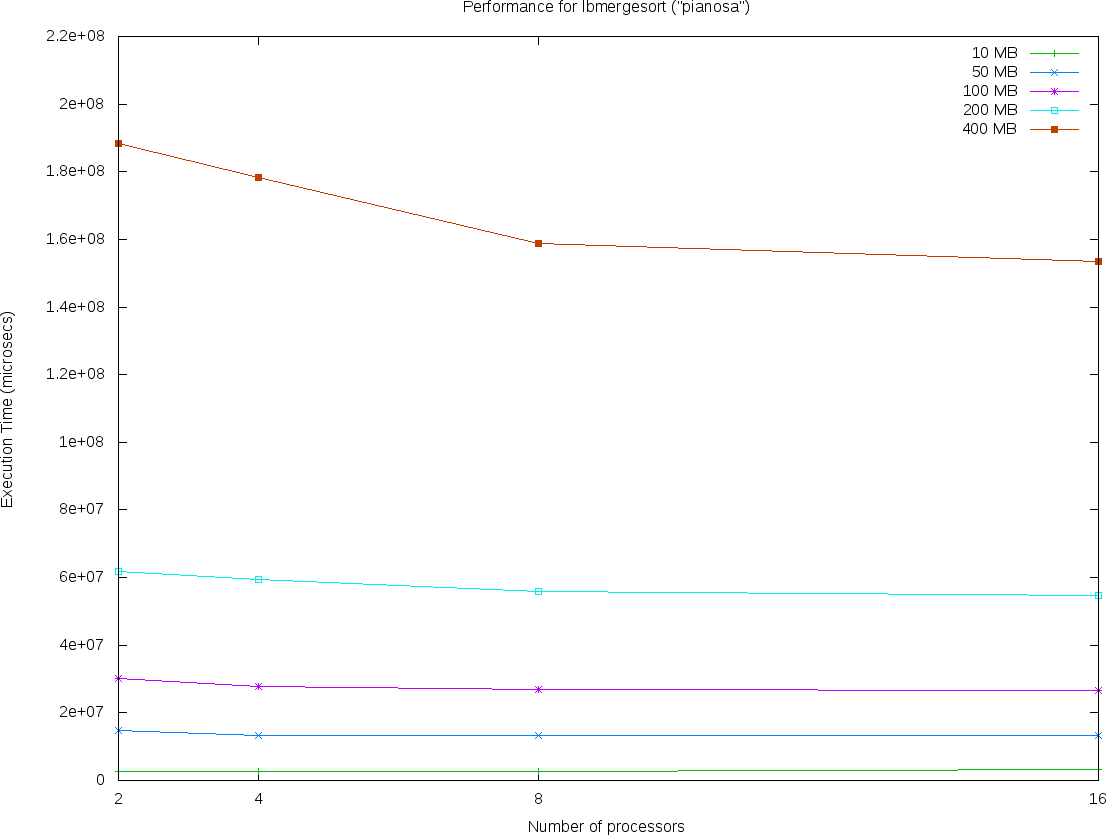
\includegraphics[width=0.4\textwidth]{results/large_lbmergesort_pianosa}}  
  	\hspace*{20pt}  
  	\subfloat[Load-Balanced Multi-Way Mergesort.]{\label{large-lbkmergesort}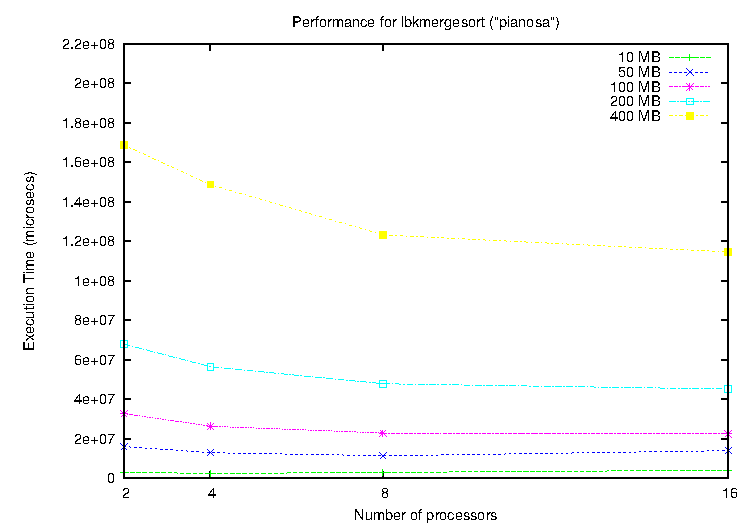
\includegraphics[width=0.4\textwidth]{results/large_lbkmergesort_pianosa}} 
  	
	\caption{Completion Time of the algorithms on Pianosa for large data sets.}
	\label{large-tc}
\end{figure}
 
\subsubsection*{Small data sets}
All our algorithms do not scale on Pianosa when the data set to sort is small (i.e. its size is of the order of hundreds of kilobytes); even worse, increasing the parallelism degree of the algorithm causes an increase of the completion time too. Figure~\ref{small-samplesort} shows the specific case of Samplesort; all other algorithms behave like Samplesort. This behavior is mainly due to the cost of communications between processes. If we model the cost of a $send$ as we did in~\ref{test-env} and if we look at the result obtained in~\ref{test-env-pianosa}, we can clearly see that the cost of sending a few kilobytes is of the order of milliseconds. On the other hand, the cost of sorting a small data set is of the order of milliseconds too (see Figure~\ref{small-sequential}; scale is not logarithmic to a better comparison with the other figures). These characteristics leads us to say, from a qualitative point of view, that the higher the parallelism degree, the higher both the number of communications and the overall time spent in sending data, so higher is even the overhead introduced by the parallelization. 

\begin{figure}[h]
	\centering
	\subfloat[Cost of sequential qsort.]{\label{small-sequential}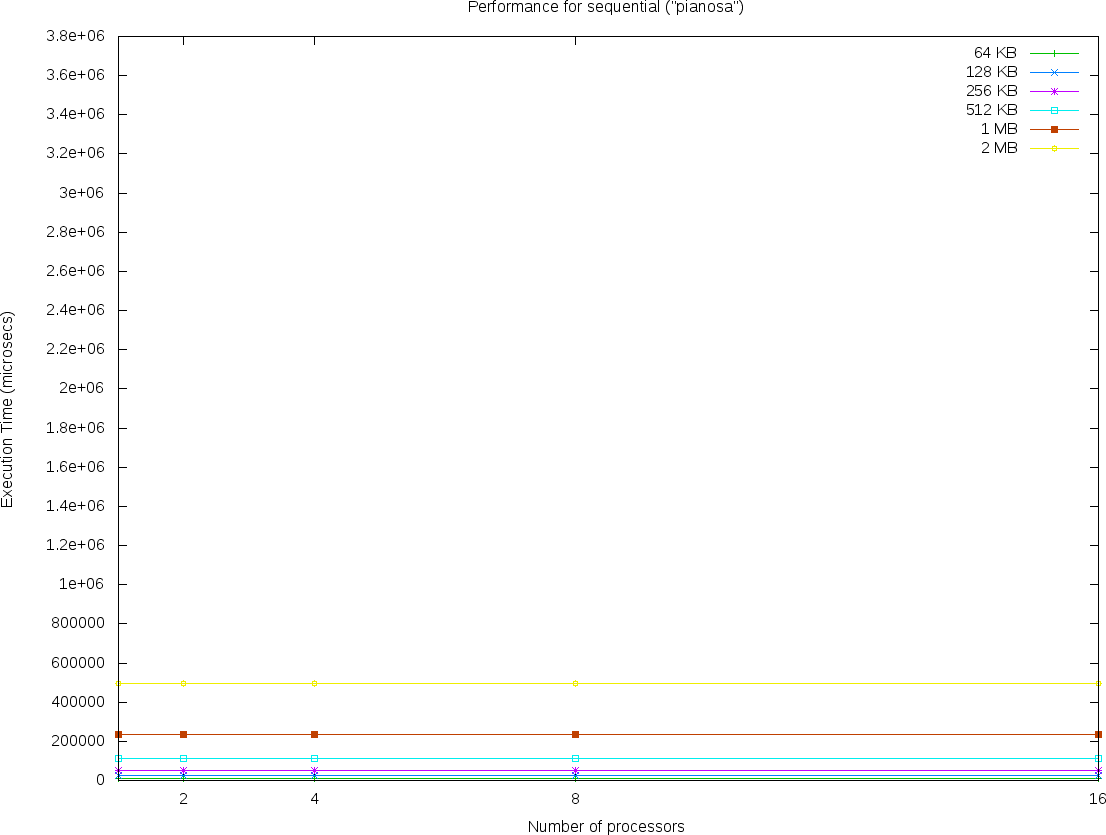
\includegraphics[width=0.4\textwidth]{results/small_sequential_pianosa}} 
	\hspace*{20pt}
  	\subfloat[Samplesort.]{\label{small-samplesort}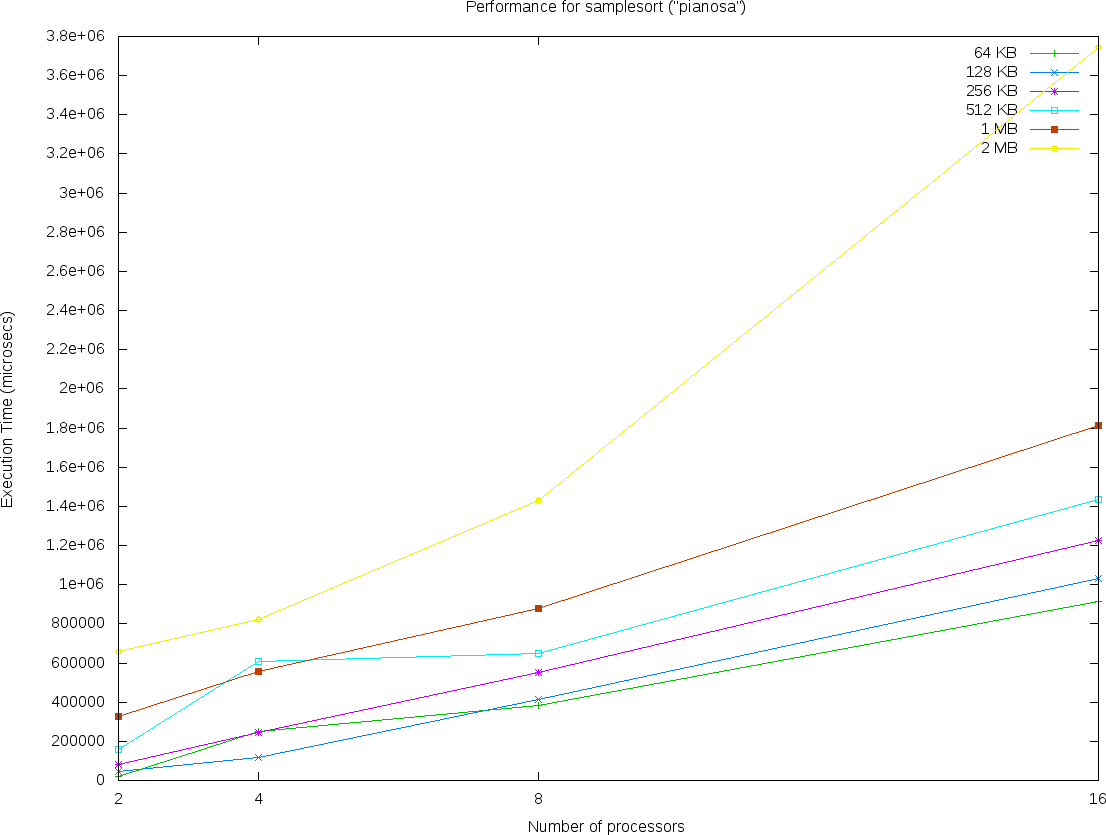
\includegraphics[width=0.4\textwidth]{results/small_samplesort_pianosa}}  
  	
  	\caption{Completion Time on Pianosa for small data sets.}
\end{figure}

